\documentclass{beamer}

\usepackage{default}
\usetheme{Warsaw}
\useinnertheme{rectangles}

\setbeamercovered{transparent}
\setbeamertemplate{bibliography item}[text]
\setbeamertemplate{sections/subsections in toc}[square]

\usepackage{graphics}
\usepackage{graphicx}
\usepackage{subfigure}

\bibliographystyle{abbrv}

\title{Cluster-Based Visualization of Web Search Results}
\author{Matthias Tilsner}
\date{March 11, 2009}

\begin{document}

\frame{\titlepage}

\frame{\tableofcontents}

\section{Introduction}
\begin{frame}{Project Domain}
	\begin{beamerboxesrounded}[shadow=true]{Web Documents}
		\begin{itemize}
			\item URL
			\item header data \begin{itemize}
				\item title
				\item meta-tags
			\end{itemize}
			\item body data \begin{itemize}
				\item textual content
				\item links
			\end{itemize}
		\end{itemize}
	\end{beamerboxesrounded}
	\vspace{5mm} \pause
	\begin{beamerboxesrounded}[shadow=true]{Search Parameters}
		\begin{itemize}
			\item query string \begin{itemize}
				\item search terms
			\end{itemize}
		\end{itemize}
	\end{beamerboxesrounded}
\end{frame}

\section{Analysis}
\begin{frame}{Visualization Techniques}
	\begin{beamerboxesrounded}[shadow=true]{Relevance to Search Terms/Query}
		\begin{itemize}
			\item \textbf{position} \cite{Einsfeld2006, Google2009, Konchady1998, Nowell1996}
			\item color \cite{Hoeber2006, Mukherjea1999, Nowell1996}
			\item size \cite{Mukherjea1996, Paulovich2008}
		\end{itemize}
		\begin{figure}[htbp]
			\begin{center}
	 			\subfigure[position \cite{Google2009}]{
					
\includegraphics[width=30mm]{images/relevance-position-Google2009.png}
				}
				\subfigure[color \cite{Hoeber2006}]{
					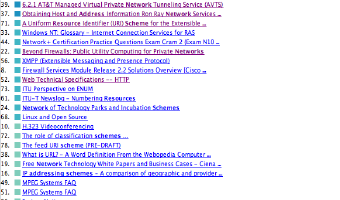
\includegraphics[width=30mm]{images/relevance-color-Hoeber2006.png}
				}
				\subfigure[size \cite{Mukherjea1996}]{
					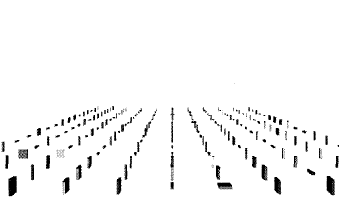
\includegraphics[width=30mm]{images/relevance-size-Mukherjea1996.png}
				}
			\end{center}
		\end{figure}
	\end{beamerboxesrounded}
\end{frame}

\begin{frame}{Visualization Techniques}
	\begin{beamerboxesrounded}[shadow=true]{Relationship of Search Results}
		\begin{itemize}
			\item position \cite{Nowell1996}
			\item connection \cite{Einsfeld2006, Mukherjea1999, Paulovich2008, Zaina2005}
		\end{itemize}
		\begin{figure}[htbp]
			\begin{center}
	 			\subfigure[position \cite{Nowell1996}]{
					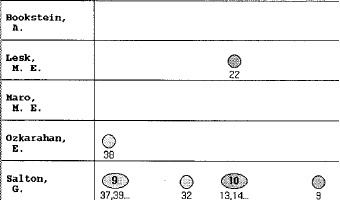
\includegraphics[width=30mm]{images/relationship-position-Nowell1996.png}
				}
				\subfigure[connection \cite{Zaina2005}]{
					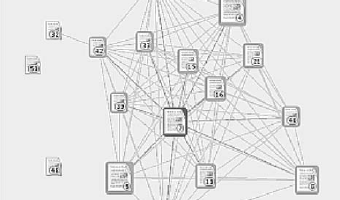
\includegraphics[width=30mm]{images/relationship-connections-Zaina2005.png}
				}
			\end{center}
		\end{figure}
	\end{beamerboxesrounded}
\end{frame}

\begin{frame}{Visualization Techniques}
	\begin{beamerboxesrounded}[shadow=true]{Similarity of Search Results}
		\begin{itemize}
			\item position \cite{Benjamin2008, Einsfeld2006, Mukherjea1996, Mukherjea1999, Paulovich2008, Rauber2000, Roussinov1999, Sebrechts1999, Tvarozek2008, Weippl2001}
		\end{itemize}
		\begin{figure}[htbp]
			\begin{center}
	 			\subfigure[position \cite{Rauber2000}]{
					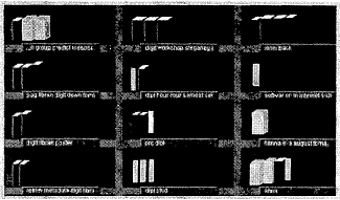
\includegraphics[width=30mm]{images/similarity-position-Rauber2000.png}
				}
			\end{center}
		\end{figure}
	\end{beamerboxesrounded}
\end{frame}

\begin{frame}{Interaction Techniques}
	\begin{beamerboxesrounded}[shadow=true]{Details on Demand}
		\begin{itemize}
			\item highlighting \cite{Weiss2001}
			\item popup \cite{Einsfeld2006}
			\item zoom \cite{Konchady1998, Mukherjea1996, Paulovich2008, Rauber2000}
		\end{itemize}
	\end{beamerboxesrounded}
	\vspace{5mm} \pause
	\begin{beamerboxesrounded}[shadow=true]{Data Refinement}
		\begin{itemize}
			\item redefine search terms \cite{Roussinov1999}
			\item search result list \cite{Einsfeld2006, Mukherjea1999}
		\end{itemize}
	\end{beamerboxesrounded}
\end{frame}

\section{Evaluation}
\begin{frame}{Current Status}
	\begin{beamerboxesrounded}[shadow=true]{Summary of Existing Research}
		\begin{itemize}
			\item either extending or abandoning conventional result lists
			\item display of all result items or a subset \begin{itemize}
				\item zoom in for structural details
				\item popup metadata
			\end{itemize}
		\end{itemize}
	\end{beamerboxesrounded}
	\vspace{5mm} \pause
	\begin{beamerboxesrounded}[shadow=true]{Assumptions}
		\begin{itemize}
			\item users: untrained, unwilling, impatient, used to conventional result lists
			\item search must be intuitive
			\item no existing solution has been widely accepted
		\end{itemize}
	\end{beamerboxesrounded}
\end{frame}

\begin{frame}{Open Issues}
	\begin{beamerboxesrounded}[shadow=true]{Interface Requirements}
		\begin{itemize}
			\item intuitive to use
			\item enables fast search success
		\end{itemize}
	\end{beamerboxesrounded}
	\vspace{5mm} \pause
	\begin{beamerboxesrounded}[shadow=true]{Beneficial Principles}
		\begin{itemize}
			\item similarity to conventional result lists
			\item usable without training \\
						$\Rightarrow$ training provides additional functionality
			\item overview-zoom-detail interaction
		\end{itemize}
	\end{beamerboxesrounded}
\end{frame}

\section{Approach}
\begin{frame}{Idea}
	\begin{beamerboxesrounded}[shadow=true]{Visualization}
		\begin{itemize}
			\item fuzzy clustering
			\item ``Concept Highlighter''-like visualization
		\end{itemize}
	\end{beamerboxesrounded}
	\vspace{5mm} \pause
	\begin{beamerboxesrounded}[shadow=true]{Interaction}
		\begin{itemize}
			\item result filtering
			\item interactive creation of customized result set
		\end{itemize}
	\end{beamerboxesrounded}	
\end{frame}

\begin{frame}{Fuzzy Clustering}
	\begin{figure}[htbp]
		\begin{center}
			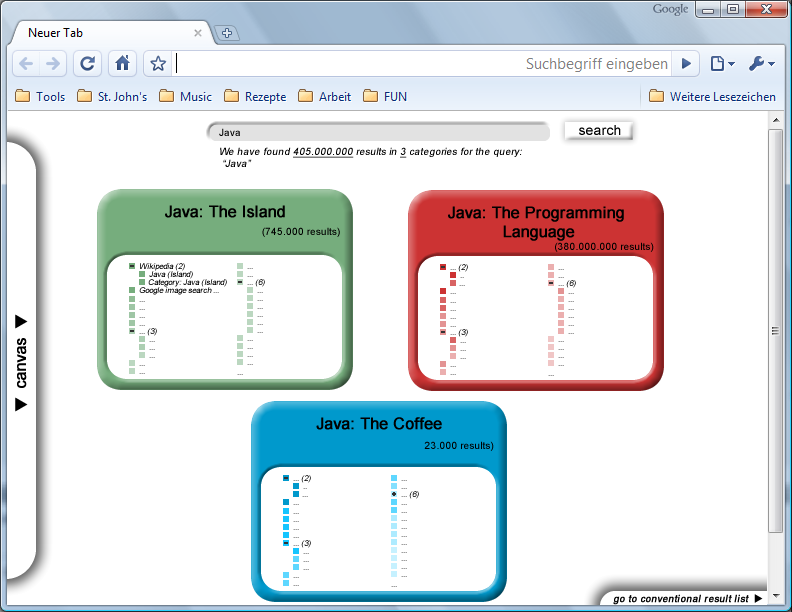
\includegraphics[height=65mm]{images/approach_fuzzy-clustering.png}
		\end{center}
	\end{figure}
\end{frame}

\begin{frame}{``Concept Highlighter''-Like Visualization}
	\begin{figure}[htbp]
		\begin{center}
			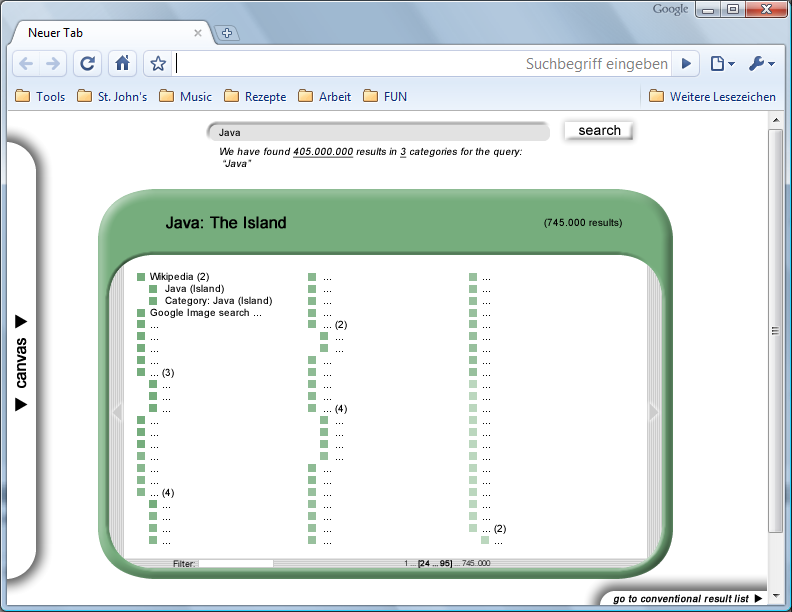
\includegraphics[height=65mm]{images/approach_resultlist.png}
		\end{center}
	\end{figure}
\end{frame}

\begin{frame}{Interactive Creation of Customized Result Sets}
	\begin{figure}[htbp]
		\begin{center}
			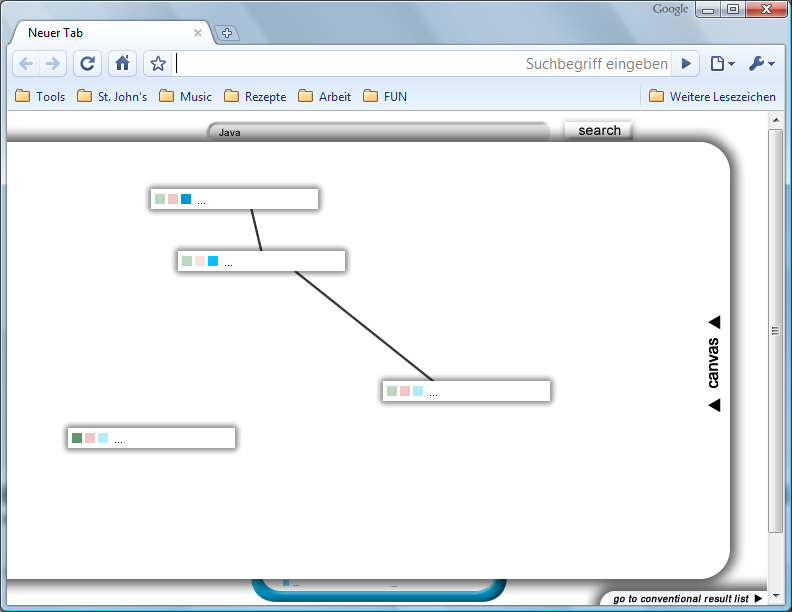
\includegraphics[height=65mm]{images/approach_interactive-creation-of-customized-result-sets.png}
		\end{center}
	\end{figure}
\end{frame}

\section{Conclusion}
\begin{frame}{Risks and Potentials}
	\begin{beamerboxesrounded}[shadow=true]{Risks}
		\begin{itemize}
			\item performance
			\item intuitivity / usability
			\item quality (clustering \& topic identification)
		\end{itemize}
	\end{beamerboxesrounded}	
	\vspace{5mm} \pause
	\begin{beamerboxesrounded}[shadow=true]{Potentials}
		\begin{itemize}
			\item fast reduction of search space
			\item easy identification of relevant results
			\item topic distinction
		\end{itemize}
	\end{beamerboxesrounded}	
\end{frame}

\begin{frame}{Outlook}
	\begin{beamerboxesrounded}[shadow=true]{Future Issues}
		\begin{itemize}
			\item customized / optimized ranking
			\item result retaining \& sharing
			\item Web Service API
			\item visualization customizing
			\item search term weighting
		\end{itemize}
	\end{beamerboxesrounded}	
\end{frame}

\begin{frame}
	\begin{beamerboxesrounded}[shadow=true]{Thank you for your attention}
		\begin{flushright}
			``If you type `Google' into Google, you can break the Internet'' \\
			- \textit{Jen (The IT Crowd)}
		\end{flushright}
	\end{beamerboxesrounded}	
\end{frame}

\begin{frame}[allowframebreaks]{References}
	\begin{tiny}
		\bibliography{literature}
	\end{tiny}
\end{frame}
\end{document}